\section{Empirical results}
Malapert uses benchmark data by Daste. For design purposes, I created my own set of randomized job lists, with $s_j, p_j \in [1, 20]$ and $d_j \in [1, 10n]$ where $n$ is the number of jobs. Here is the Python code used:

\lstset{language=Python}
\begin{lstlisting}
import random

random.seed(None)

for i in range(11, 20) + range(10,100,10):
    for j in range(1, 10):
        with open( "data_" + str(i) + "_" + str(j), "wb") as csvfile:
            csvwriter = csv.writer(csvfile, delimiter=",")
            csvwriter.writerow(['s_j', 'p_j', 'd_j'])
            for job in range(i):
                csvwriter.writerow([random.randrange(1,20), random.randrange(1,20), random.randrange(1,5*i)])
        csvfile.close()
\end{lstlisting}

CSV files can be read in with \texttt{IloCsvReader} and \texttt{IloCsvLine}.

\subsection{Comparison of CPU time used by various models}
Figure \ref{fig:comp_times} shows the CPU time used by the models. Ten sample
job sets are used per number of jobs, represented as $\left[\{10.0, \dots, 10.9\},
\{11.0, \dots, 11.9\},\dots \right]$ on the horizontal axis. The models were run
on an i7 Q740 CPU, which has $2 \times 4$ cores. Cplex supports multithreading
and as such, elapsed wall clock time is significantly lower in most cases.
\begin{figure}
\centering

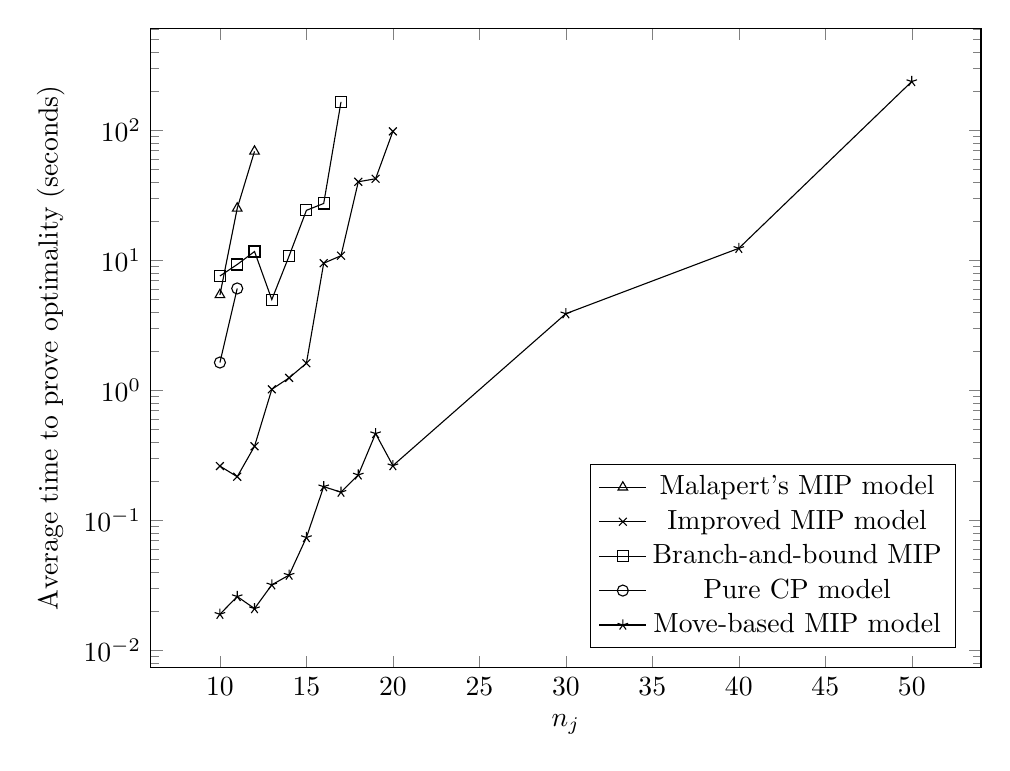
\begin{tikzpicture}
  \begin{semilogyaxis}[xlabel=$n_j$, ylabel=Average time to prove optimality (seconds), width=\textwidth,
  height=0.8\textwidth,legend pos=south east]
  \addplot[color=black, mark=triangle ] coordinates { % MIP model times
  (10, 5.441)
  (11, 25.18)
  (12, 69.05)
  };   \addlegendentry{Malapert's MIP model}

  \addplot[color=black, mark=x ] coordinates { % MIP model times
  (10, 0.262)
  (11, 0.217)
  (12, 0.372)
  (13, 1.02)
  (14, 1.25)
  (15, 1.62)
  (16, 9.52)
  (17, 10.88)
  (18, 40.3)
  (19, 42.5)
  (20, 98.415)
  };   \addlegendentry{Improved MIP model}

  \addplot[color=black, mark=square] coordinates {
(10, 7.59)
(11, 9.31)
(12, 11.72)
(13, 5)
(14, 10.83)
(15, 24.28)
(16, 27.44)
(17, 165.82)
  };
  \addlegendentry{Branch-and-bound MIP}
  \addplot[color=black, mark=o] coordinates {
(10, 1.64)
(11, 6.09)
};
  \addlegendentry{Pure CP model}
  \addplot[color=black, mark=star] coordinates {
(10, 0.019)
(11, 0.026)
(12, 0.021)
(13, 0.032)
(14, 0.038)
(15, 0.074)
(16, 0.182)
(17, 0.165)
(18, 0.224)
(19, 0.466)
(20, 0.264)
(30, 3.895)
(40, 12.403)
(50, 238)
};
  \addlegendentry{Move-based MIP model}
  \end{semilogyaxis}
\end{tikzpicture}

\caption{Comparison of CPU time used by different models to find an optimal
schedule and prove its optimality.}
\label{fig:comp_times}
\end{figure}



